\section{Theorie} \label{sec:Theorie}

Im Folgenden sollen die theoretischen Grundlagen des Geiger-Müller-Zählrohrs erläutert werden.

\subsection{Aufbau des Zählrohrs}

    \begin{figure}
      \centering
      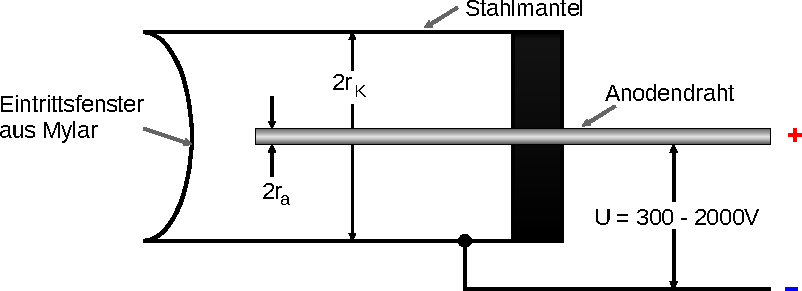
\includegraphics[width=0.75\textwidth]{content/img/Abb_1.pdf}
      \caption{Aufbau des Geiger-Müller-Zählrohrs \cite{versuchsanleitung}.}
      \label{fig:abb1}
    \end{figure}

    Das Geiger-Müller-Zählrohr besteht aus einem zylinderförmigen, negativ geladenen Rohr mit Radius $r_\text{k}$,
    in dessen Mitte sich ein positiv geladener Draht mit Radius $r_\text{a}$ befindet.
    Der Zylindermantel stellt eine Kathode dar und der Draht eine Anode.
    Zwischen Anode und Kathode befindet sich ein elektrisches Feld,
    welches aufgrund der Symmetrie des Zählrohrs radialsymmetrisch vom Draht nach außen gerichtet ist.
    Für die elektrische Feldstärke ergibt sich
    \begin{equation}
        E(r) = \frac{U}{r \symup{ln}\left(\frac{r_\text{k}}{r_\text{a}}\right)} \; .
    \end{equation}
    An den Zylindermantel und den Draht ist die Spannung $U$ angeschlossen.
    Durch ein Eintrittsfenster im Deckel der Röhre können Teilchen in das Innere des Zylinders
    gelangen, welches mit einem Gasgemisch, in diesem Fall Halogen, gefüllt ist.

\subsection{Wirkungsweise}

    Das Geiger-Müller-Zählrohr wird zur Bestimmung der Intensität ionisierender Strahlung genutzt.\\
    Wenn ein geladenes Teilchen durch das Eintrittsfenster,
    welches aus einem sehr durchlässigen Material besteht,
    in das Innere des Zylinders gelangt, ionisiert es Gasatome.
    Dieser Vorgang wird Primärionisation genannt.
    So entstehen freie Elektronen,
    welche sich zum positiv geladenen Draht in der Mitte bewegen und durch diesen abfließen.
    Es entsteht ein Ionisationsstrom. \\
    In Abhängigkeit der Spannung kommt es zu verschiedenen Reaktionen.
    In \autoref{fig:abb2} sind diese in verschiedene Bereiche von \RMN{1} bis \RMN{5} unterteilt.\\

    \begin{figure}
      \centering
      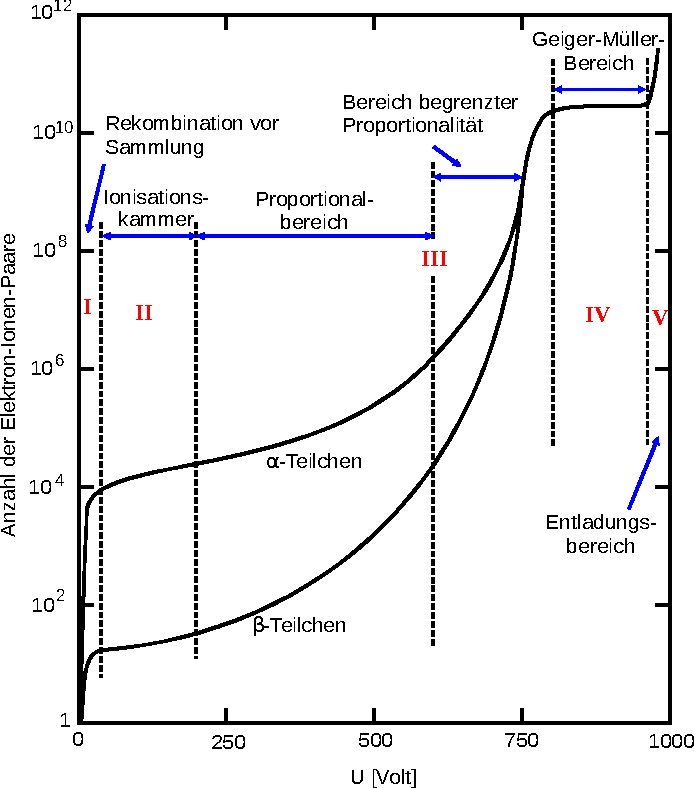
\includegraphics[width=0.75\textwidth]{content/img/Abb_2.pdf}
      \caption{Anzahl der erzeugten Elektron-Ionenpaare in Abhängigkeit der Spannung mit eingezeichneten Bereichen \cite{versuchsanleitung}.}
      \label{fig:abb2}
    \end{figure}

    Wenn die Spannung klein ist, findet im Bereich \RMN{1} Rekombination statt,
    und nur ein Teil der freien Elektronen gelangt zum Draht.
    In diesem Bereich steigt die Zahl der Elektronen-Ionen-Paare sehr stark an.\\
    \\
    Im Bereich \RMN{2} ist die Spannung etwas größer und damit auch die elektrische Feldstärke,
    sodass alle freien Elektronen aus der Primärionisation zum Draht gelangen.
    In diesem Bereich operierende Geräte werden \textit{Ionisationskammern} genannt.\\
    \\
    Der Bereich \RMN{3} wird in \textit{Proportionalitätsbereich} und \textit{Bereich begrenzter Proportionalität} aufgeteilt.
    Die Spannung nimmt weiter zu, sodass die freien Elektronen genug Energie haben,
    um die Gasatome anzuregen.
    Es folgt die Stoßionisation, bei der weitere freie
    Elektronen mit ausreichend hoher Energie freigesetzt werden,
    sodass eine Lawine an freien Elektronen entsteht.
    Anhand der Ladungsimpulse, die beim Auftreffen der Elektronen auf dem Draht entstehen,
    kann mit der Proportionalitätsbeziehung zur Energie
    eine Abschätzung für die Teilchenzahl getroffen werden.
    Je höher jedoch die Spannung steigt,
    desto mehr Teilchen treffen auf den Draht und die Proportionalität wird begrenzt.
    In diesem Bereich steigt die Zahl der Elektronen-Ionen-Paare wieder stark an.\\
    \\
    Der eigentliche Arbeitsbereich des Geiger-Müller-Zählrohrs ist Bereich \RMN{4}.
    Die Spannung ist jetzt so groß,
    dass bei der Ionisation zusätzlich zu Elektronen auch UV-Photonen entstehen,
    welche sich unbeinflusst vom elektrischen Feld bewegen können.
    Es entstehen Elektronenlawinen im gesamten Zählrohr.
    Der Ladungsimpuls, welcher am Anodendraht gemessen wird, ist nun unabhängig vom einfallenden Teilchen.
    Zu diesem Zeitpunkt bleibt die Zahl der Elektronen-Ionen-Paare nahezu konstant.
    Entsprechend wird dieser Bereich \textit{Plateau} genannt.
    Dieses ist in der Charakteristik in \autoref{fig:abb4} zu sehen,
    welche den Bereich \RMN{4} aus \autoref{fig:abb2} vergrößert darstellt.

    \begin{figure}
      \centering
      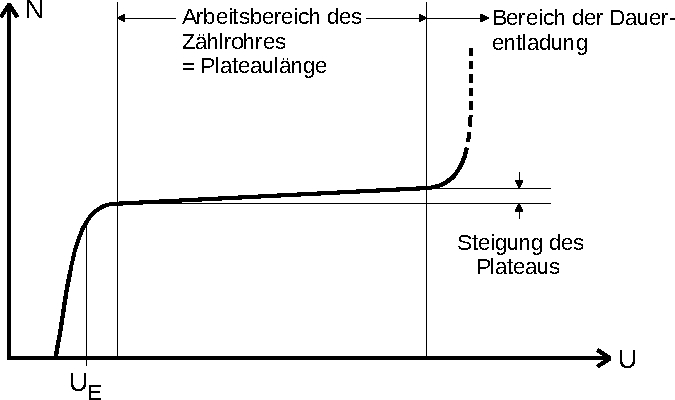
\includegraphics[width=0.75\textwidth]{content/img/Abb_4.pdf}
      \caption{Vergrößerte Darstellung des Plateau-Bereichs \cite{versuchsanleitung}.}
      \label{fig:abb4}
    \end{figure}

    Wenn die Spannung noch höhere Werte annimmt,
    kommt es in Bereich \RMN{5} zu einer Dauerentladung,
    welche eine hohe Stromdichte hervorruft.
    In diesem Bereich wird das Geiger-Müller-Zählrohr zerstört.\\
    \\
    Der mittlere Zählrohrstrom, also die Ladungsmenge,
    die beim Auftreffen der Teilchen auf dem Draht freigesetzt wird, kann durch
    \begin{align}
        \bar{I} &\approx \frac{1}{\tau} \int_0^{\tau}{\frac{U(t)}{R}} \symup{d}t \\
        \bar{I} &\approx \frac{\symup{\Delta}Q}{\symup{\Delta}t} Z
    \end{align}
    berechnet werden.
    Dabei ist $\symup{\Delta}Q$ die Ladungsmenge,
    welche in einer Zeit $\symup{\Delta}t$ von $Z$ Teilchen übertragen wurde.
    Für $Z$ gilt
    \begin{equation}
      \label{eqn:Teilchenzahl}
      Z = \frac{I}{e_0 N} \; .
    \end{equation}

\subsection{Totzeit und Nachentladung}

    Die positiven Ionen,
    die bei den Reaktionen eines einfliegenden Teilchens mit den Gasatomen entstehen,
    fließen nicht durch den Draht ab.
    Es baut sich ein Ionenschlauch auf, also ein Gebiet positiver Raumladung,
    welche das elektrische Feld so beeinflusst, dass für eine Zeit $T$ keine Stoßionisation stattfindet.
    Diese Zeit $T$ wird Totzeit genannt.
    Während dieser Zeit wird ein eintreffendes Teilchen nicht regristriert.
    Nach der Totzeit folgt eine Erholungszeit $T_\text{E}$,
    in der schwächere Ausgangsimpulse regristriert werden (vgl. \autoref{fig:abb3}).

    \begin{figure}
      \centering
      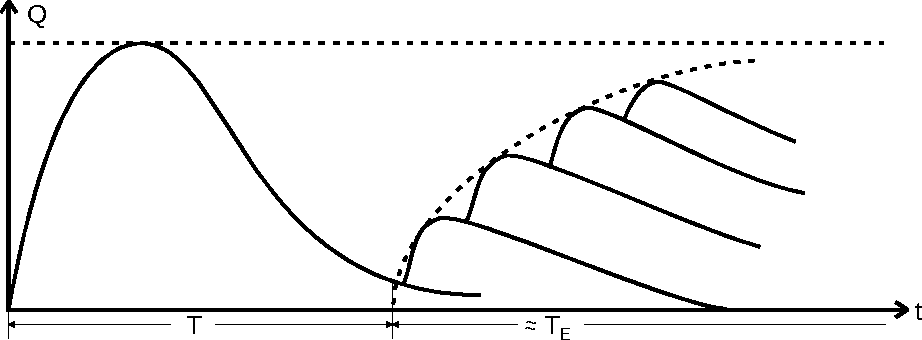
\includegraphics[width=\textwidth]{content/img/Abb_3.pdf}
      \caption{Tot- und Erholungszeit eines Zählrohrs, dargestellt im Ladungs-Zeit-Diagramm \cite{versuchsanleitung}.}
      \label{fig:abb3}
    \end{figure}

    Die Totzeit kann näherungsweise mithilfe der Gleichung
    \begin{equation}
      \label{eqn:totzeit}
      T \approx \frac{N_1 + N_2 - N_{1+2}}{2 N_1 N_2}
    \end{equation}
    berechnet werden, wenn $T^2 N_i ^2 \ll 1$ gilt.
    $N_1$ bezeichnet die Zählrate, die für ein erstes Präparat gemessen wird,
    $N_{1+2}$ die Zählrate, die gemessen wird, wenn ein zweites Präparat hinzugefügt wird,
    und $N_2$ die Zählrate für das zweite Präparat, nachdem das erste entfernt wurde.\\
    \\
    Die positiven Ionen werden zur negativ geladenen Kathode gezogen,
    wodurch sich der Ionenschlauch auflöst und wieder Stoßionisation möglich ist.
    Wenn die Ionen auf der Kathode auftreffen,
    lösen sie Elektronen, sogenannte Sekundärelektronen, aus dem Material.
    Dieser Vorgang wird Nachentladung genannt und sorgt dafür,
    dass mehrere Ausgangsimpulse entstehen, wenn ein Teilchen durch die Röhre geflogen ist,
    welche im zeitlichen Abstand $T_\text{L}$ voneinander liegen.
    Diese Zeit $T_\text{L}$ ist länger als die eigentliche Totzeit.
    Um die Nachentladung zu minimieren, werden zum Gasgemisch Alkoholdämpfe hinzugefügt,
    welche bei Ionisation eine zu geringe Energie haben, um ihrerseits ionisieren zu können.\\
    \\
    Im Übergang von Bereich \RMN{4} zu \RMN{5} nimmt die Zahl der Nachentladungen stark zu,
    welche die Ursache für die Dauerentladung des Geiger-Müller-Zählrohrs sind.


    %Ansprechvermögen des Zählrohrs
